\documentclass[12pt, oneside]{article}%Tipo de documento y tamaño de letra%
\usepackage[spanish]{layout}
%\usepackage{hyperref}
\usepackage{color,graphicx}%Para poder incertar graficas%
\usepackage{graphics}
\usepackage{amsmath,amssymb}%Insertar unos simbolos matematicos especiales%
\usepackage{setspace}
%\usepackage{empheq}
%\usepackage{multicol}
\onehalfspacing
%\usepackage[mathscr]{euscript}%Tipo especial de letra%
\usepackage[utf8]{inputenc}%Para las tildes
\usepackage[spanish,activeacute]{babel} %Todo en Español
%\usepackage{multicol}
\pagestyle{empty}
%\usepackage{spalign}  %SISTEMAS DE ECUACIONES%
%\usepackage{array}
\usepackage{layout}
\usepackage{manfnt}
\usepackage{float}
\usepackage{CJKutf8}
%\usepackage{xeCJK}
%\setCJKsansfont{IPAexMincho}
\usepackage{mathrsfs}
\usepackage{listings}
\usepackage{xcolor}

\definecolor{codegreen}{rgb}{0,0.6,0}
\definecolor{codegray}{rgb}{0.5,0.5,0.5}
\definecolor{codepurple}{rgb}{0.58,0,0.82}
\definecolor{backcolour}{rgb}{256,256,256}

\lstdefinestyle{mystyle}{
    backgroundcolor=\color{backcolour},   
    commentstyle=\color{codegreen},
    keywordstyle=\color{codegreen},
    numberstyle=\tiny\color{codegray},
    stringstyle=\color{codepurple},
    basicstyle=\ttfamily\footnotesize,
    breakatwhitespace=false,         
    breaklines=true,                 
    captionpos=b,                    
    keepspaces=true,                 
    numbers=left,                    
    numbersep=5pt,                  
    showspaces=false,                
    showstringspaces=false,
    showtabs=false,                  
    tabsize=2
}


\def\Car{{\textsf{Car}}}
\def\Ring{{\mathcal R}}
\def\Z{{\mathbb Z}}
\def\R{{\mathbb R}}

\def\F{{\mathbb F}}
\def\Wolfram{{\emph{Mathematica}\textsuperscript{\textregistered} }}

\usepackage{picinpar}
\setlength{\oddsidemargin}{0pt}
\setlength{\topmargin}{0pt}
\setlength{\headheight}{0pt}
\setlength{\headsep}{0pt}
\setlength{\textheight}{24cm}
\setlength{\textwidth}{17cm}
\setlength{\marginparsep}{0pt}
\setlength{\marginparwidth}{0pt}
\setlength{\footskip}{1cm}


\begin{document}
\setlength{\parindent}{0cm}%EL ANCHO DE LA SANGRIA DE AQUÍ EN ADELANTE%
\hoffset-0.46cm
\voffset-1.46cm

\begin{window}[0,l,{
\includegraphics[scale=0.6]{logo.jpg}},]
\Large  \hspace{0.5cm}\textsf{Universidad Nacional de Colombia} \\
\textcolor{white}{\tiny.}  \Large \hspace{0.6cm} \textsf{Departamento de Matemáticas} \\
\textcolor{white}{\tiny.}   \large\hspace{1.6cm}\textsf{Introducción a la optimización}\\
\textcolor{white}{\tiny.}   \large \hspace{2.6cm}\textsf{Tarea 5} \normalsize (I-2022)\\
\end{window}

\vspace{0.5cm}
\normalfont
\textsf{} 
\normalsize
Daniel Santiago Pardo Gomez\\
David Antonio Garzón Avendaño
\dotfill
\begin{enumerate}
\item (3.2) Level sets of convex, convave, quasiconvex, and quasiconcave functions.  Some level sets of a function $f$ are shown below. The curve labeled 1 shows $\{x | f(x) = 1\}$, etc.
\begin{center}
    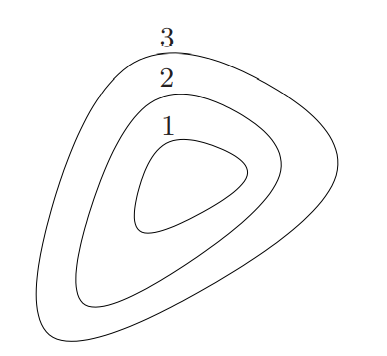
\includegraphics[scale=0.6]{img1.png}
\end{center}
Could $f$ be convex (concave, quasiconvex, quasiconcave)? Explain your answer. Repeat for the level curves shown below.
\begin{center}
    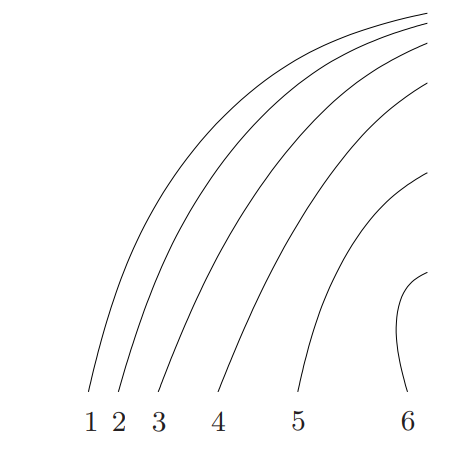
\includegraphics[scale=0.5]{img2.png}
\end{center}

\textbf{Respuesta}: \\
En el caso de la primera imagen si asumimos que las demás curvas de nivel guardan regularidad con las mostradas en la imagen, entonces, la función $f$ sería convexa y después cuasiconvexa puesto que en la imagen podemos observar que a medida que $\alpha$ aumenta su curva de nivel "rodea" a las anteriores, esto indica que las imágenes de una combinación convexa serían menores a las de sus extremos y como sabemos que esta idea corresponde a la de una función convexa, se podría dar este caso.\\
Para el caso de la segunda imagen sucede una situación similar, pero para ésta se puede tener el caso de concavidad, es decir, las curvas de nivel de los valores menores "rodean" a las mayores y aplicando un razonamiento análogo observamos que esta función podría ser cóncava y cuasicóncava.

\item (3.4) Show that a continuous function $f: R^n \leftarrow R$ is convex if and only if for every line segment, its average value on the segment is less than or equal to the average of its values at the endpoints of the segment: For every $x, y \in R^n$.

$$ \int_0^1 f(x+\lambda(y-x)) d\lambda \leq \frac{f(x) + f(y)}{2}$$
\textbf{Respuesta}: \\
$\Rightarrow$ Supongamos que $f(x)$ es una función continua y convexa, entonces podemos usar la desigualdad de Jessen para escribir la función de la siguiente manera: 
$$f(x + \lambda(y-x)) \leq f(x) + \lambda(f(y) - f(x)) $$

Para $0\leq \lambda \leq 1$. Integrando a ambos lados desde 0 hasta 1 tenemos:

$$ \int_0^1 f(x+\lambda(y-x)) d\lambda \leq \int_0^1 f(x) + \lambda(f(y) - f(x)) = \frac{f(x) + f(y)}{2} $$
$\Leftarrow$ Contradición: Supongamos que se tiene $ \int_0^1 f(x+\lambda(y-x)) d\lambda \leq \frac{f(x) + f(y)}{2}$ y que $f(x)$ no es convexa. Entonces para algún 字 con $0\leq \text{字} \leq 1$ se tiene que: 
$$f(\text{字}x + (1-\text{字}y)) > \text{字}f(x) + (1-\text{字})f(y)$$

Ahora tomemos la siguiente función:
$$H(\theta) = f(\theta + (1-\theta)y) - \theta f(x) -(1-\theta)f(y)$$

Esta función es continua pues $f$ es continua por hipotesis. Ahora note que para $\theta = 0$ y $\theta = 1$ H es igual a 0 y 字 es positivo. Ahora tomemos $\alpha$ como el mayor cruce por 0 de H por debajo de 字 y tomemos a $\beta$ como el menor cruce por 0 de H por encima de 字. Definimos $u = \alpha x+ (1- \alpha)y $ y $v = \beta x+ (1- \beta)y$. Entonces para el intervalo $(\alpha, \beta)$ tenemos: 

$$f(\theta x + (1-\theta y)) > \theta f(x) + (1- \theta)f(y)$$

Por lo que para $0 \leq \theta \leq 1$ tenemos:
$$f(\theta u + (1-\theta v)) > \theta f(u) + (1- \theta)f(v)$$
Ahora integrando desde 0 hasta 1 tenemos: 

$$\int_0^1 f(\theta u + (1-\theta v)) d\theta > \int_0^1  \theta f(u) + (1- \theta)f(v)d\theta = \frac{f(u) + f(v)}{2}$$

Note que esto implica que el promedio de f en el intervalo $[u,v]$ es mayor que el promedio de los valores en los extremos. 

\item (3.6) \textit{Functions and epigraphs}. When is the epigraph of a function a halfspace? When is the epigraph of a function of a convex cone? When is the epigraph of a function a polyhedron?\\ \\
\textbf{Respuesta}: \\
\begin{itemize}
    \item \textbf{Semiespacio:} Para este caso es necesario que la función sea afín, es decir, que pueda escribirse de la forma $f(x)=Ax+b$.
    \item \textbf{Cono convexo:} En este caso resulta necesario que la función cumpla que $f(\alpha x)=\alpha f(x)$ con $\alpha \geq 0$
    \item \textbf{Poliedro:} Finalmente para este caso tendríamos que la función sea de la forma
    $$f(x)=\begin{cases}
    A_1x+b_1 & \text{si } x\in P_1\\
    \vdots & \vdots\\
    A_nx+b_n & \text{si } x\in P_n\\
    \end{cases}
    $$
    Donde $\{P_1,\cdots,P_n\}$ es una partición del dominio de $f$\\
\end{itemize}
\item (3.13) \textit{Kullback-Leibler divergence and the information inequality}. Let $D_{kl}$ be the Kullback-Leibler divergence, as defined in (3.17). Prove the \textit{information inequality}: $D_{kl}(u,v) \geq 0$ for all $u,v \in R_{++}^n.$ Also show that $D_{kl}(u,v) = 0$ if and only if $u=v$.

\textit{Hint}. The Kullback-Leibler divergence can be expressed as:

$$ D_{kl}(u,v) = f(u) - f(v) - \nabla f(v)^T(u-v),$$

where $f(v) = \sum_{i=1}^n v_i \log (v_i)$ is the negative entropy of $v$.\\ \\
\textbf{Respuesta}: 

Sean $u,v\in \mathbb{R}_{++}^n$ cualesquiera, dado que la entropía negativa es convexa en el dominio dado, por la condición de primer orden tenemos que:
\begin{align*}
    f(u)\geq &f(v)+\nabla f(v)^T(u-v)\\
    f(u)-f(v)-\nabla f(v)^T(u-v)\geq 0\\
\end{align*}
Entonces $D_{kl}(u,v) \geq 0$.
$\Rightarrow$ Supongamos ahora que $u=v$, entonces:
$$f(u) - f(v) - \nabla f(v)^T(u-v)=f(u) - f(u) - \nabla f(v)^T(u-u)=0$$
$\Leftarrow$ Supongamos que:
$$f(u) - f(v) - \nabla f(v)^T(u-v)=0$$
Note que:
$$\nabla f(v)^T(u-v)=\sum_{i=1}^n (1+\log (v_i))(u_i-v_i)$$
Pero como $1+\log (x)>0$ para todo $x>0$ entonces de debe cumplir que $u=v$.
\item (3.16) For each of the following functions determine whether it is convex, concave, quasiconvex, or quasiconcave. \\

\textbf{Respuesta}: 

\begin{itemize}
    \item $f(x) = e^x - 1$ on $R$.
    Note que $f''(x) = e^x > 0$, así que usando la condición de segundo orden tenemos que la función es estrictamente convexa, lo que implica que es cuasiconvexa y no cuasicóncava 
 
    
    \item $f(x_1,x_2) = x_1x_2$ on $R_{++}^2$
    vamos a usar la condición de segundo orden, así que procedemos a sacar el Hessiano de f. 
    
    $$ \nabla^2 f = \begin{pmatrix}
                    0 & 1\\
                    1 & 0
                    \end{pmatrix} $$
    
    Note que los autovalores de la matriz son $1$ y $-1$, por lo que no es ni semidefinida positiva ni semidefinida negativa. Lo que implica que la función no es ni cóncava no convexa. 
    
    Por otro lado la función tampoco es cuasiconvexa, note que:  $\nabla f =  \begin{pmatrix} x_2\\ x_1 \end{pmatrix} $ 
    Por lo que: 
    $$\nabla f(x)^T(x-y) = \begin{pmatrix} x_2 & x_1 \end{pmatrix} \begin{pmatrix} y_1 - x_1 \\ y_2 - x_2 \end{pmatrix} = x_2(y_1-x_1) + x_1(y_2-x_2)$$
    
    Tomando $x=(6,2)$ y $y=(4,3)$ tenemos $f(x) = f(y)$ y: 
    $$x_2(y_1-x_1) + x_1(y_2-x_2) = 2(4-6) + 6(3-2)= -4 + 6 = 2$$ 
    Así $\nabla f(x)^T(x-y) > 0$. 
    
    Por último note que los superlevel sets de esta función son de la forma 
    
    $\{ (x_1,x_2) \in R{++}^2 : x_1x_2 > \alpha \}$ son convexos, por lo que la función es cuasicóncava.
    
    \item $f(x_1,x_2) = 1/(x_1x_2)$ on $R{++}^2$
    Sacando el Hessiano tenemos:
    $$ \nabla^2 f(x) = \frac{1}{x_1x_2} \begin{pmatrix} \frac{2}{x_1^2} &  \frac{1}{x_1x_2} \\ \frac{1}{x_1x_2} &  \frac{2}{x_2^2} \end{pmatrix}$$
    Note que como $x \in R_{++}^2$ tenemos que $\nabla^2 f(x) \succeq 0 $
    
    Veamos que la función es no cuasicóncava: 
    $$\nabla f(x)^T(x-y) = \begin{pmatrix} \frac{-1}{x_1^2x_2} & \frac{-1}{x_1x_2^2} \end{pmatrix} \begin{pmatrix} y_1 - x_1 \\ y_2 - x_2 \end{pmatrix} = \frac{-1}{x_1^2x_2} (y_1 - x_1)  + \frac{-1}{x_1x_2^2} (y_2 - x_2)$$ 
    Note que esto no siempre es menor o igual a 0. 
    
    \item $f(x_1,x_2) = x_1/x_2$ on $R_{++}^2$
    Sacando el Hessiano tenemos:
    $$ \nabla^2 f(x) = \begin{pmatrix} 0 &  \frac{-1}{x_2^2} \\ \frac{-1}{x_2^2} &  \frac{2x_1}{x_2^3} \end{pmatrix} $$ Note que esto no es ni semidefinida positivo ni semidefinida negativo, por lo que la función no es cóncava y tampoco convexa. 
    Por otro lado note que los sublevel y superlevel sets son de la siguiente forma: 
    $$\{(x_1,x_2): \frac{x_1}{x_2} \leq \alpha\} = \{(x_1,x_2): x \leq \alpha y\}$$
    $$\{(x_1,x_2): \frac{x_1}{x_2} \geq \alpha\} = \{(x_1,x_2): x \geq \alpha y\}$$
    Ambos son hiperplanos, por lo que la función es tanto cuasicóncava como cuasiconvexa. 
    
    \item $f(x_1,x_2) = x_1^2/x_2$ on $R \times R_{++}$
    Sacando el Hessiano tenemos:
    $$ \nabla^2 f(x) = \begin{pmatrix} \frac{2}{x_2} & \frac{-2x_1}{x_2^2} \\\frac{-2x_1}{x_2^2} & \frac{2x_1}{x_2^3} \end{pmatrix} = \left(\frac{2}{x_2}\right) \begin{pmatrix} 1 \\ \frac{-2x_1}{x_2} \end{pmatrix} \begin{pmatrix} 1 &  \frac{-2x_1}{x_2} \end{pmatrix} \succeq 0$$
    Luego la matriz es concavexa y cuasiconvexa. Además esta función no es cuasiconvexa. 
   
    
    \item $f(x_1,x_2) = x_1^{\alpha}x_2^{1-\alpha},$ where $0 \leq 1$ on $R{++}^2$
    Sacando el Hessiano tenemos:
    $$ \nabla^2 f(x) = \begin{pmatrix} \alpha(\alpha-1)x_1^{\alpha-2}x_2^{1-\alpha} & \alpha(1- \alpha)x_1^{\alpha-1}x_2^{-\alpha} \\ \alpha(1- \alpha)x_1^{\alpha-1}x_2^{-\alpha} & (1-\alpha) (-\alpha)x_1^{\alpha}x_2^{-\alpha-1}\end{pmatrix}$$
    Sin embargo note que esta matriz se puede escribir de la siguiente manera
    $$-\alpha(1-\alpha)x_1^\alpha x_2^{1-\alpha} \begin{pmatrix} \frac{1}{x_1} \\ \frac{-1}{x_2}\end{pmatrix}
    \begin{pmatrix} \frac{1}{x_1} & \frac{-1}{x_2} \end{pmatrix} \preceq 0$$
    Por lo tanto $f$ es cóncava y cuasicóncava. Además f no es cuasiconvexa. 
\end{itemize}

\item (3.20) \textit{Composition with an affine function}. Show that the following functions $f: R^n \rightarrow R$ are convex. 

\begin{enumerate}
    \item $f(x) = \|Ax-b\|$, where $A \in R^{mxn}, b \in R^m$, and $\|\cdot\|$ is a norm on $R^m$.\\
    \textbf{Respuesta}: \\
    Dado que la norma $\|\|$ es convexa y $Ax+b$ es una función afín entonces $f$ es una función convexa.
    
    \item $f(x) = -(\det(A_0 + x_1A_1 + \cdots + x_nA_n))^{1/m}$, on $\{x | A_0 + x_1A_1 + \cdots + x_nA_n \succ 0 \},$ where $A_i \in S^m$.\\
    \textbf{Respuesta}: \\
    Sabemos por el ejercicio (3.18) que la función $h(X)=-(\det X)^{1/m}$ es convexa, después como $A_0 + x_1A_1 + \cdots + x_nA_n$ es una función afín entonces tenemos que $f$ es convexa
    
    \item $f(X) = \textsf{tr}(A_0 + x_1A_1 + \cdots + x_nA_n)^{-1}, $ on $\{ x | A_0+x_1A_1 + \cdots + x_nA_n \succ 0\}$, where $A_i \in S^m$. (Use the fact that $tr(X^{-1})$ is convex on $S_{++}^m$; see exercise 3.18).\\
    \textbf{Respuesta}: \\
    De manera análoga al punto anterior, dado que tenemos que $\textsf{tr}(X^{-1})$ es convexa en las matrices semidefinidas positivas y una función afín  $A_0 + x_1A_1 + \cdots + x_nA_n$, entonces $f$ es convexa.
\end{enumerate}
\item (3.21) \textit{Pointwise maximum and supremum}. Show that the following functions $f: R^n \rightarrow R$ are convex. \\\\
\textbf{Respuesta}:
\begin{enumerate}
    \item $f(x) = max_{i=1m,\cdots,k} \|A^{(i)}x- b^{(i)}\|$, where $A^{(i)} \in R^{m \times n}, b^{(i)} \in R^m$ and $\|\cdot\|$ is a norm on $R^m$.\\
    Como vimos en el punto (3.20.a) $\|A^{(i)}x- b^{(i)}\|$ es una función convexa para cualquier $i$ y puesto que $f$ halla el máximo entre funciones convexas, tenemos que $f$ es también convexa.
    \item $f(x) = \sum_{i=1}^r |x|_{[i]}$ on $R^n$, where $|x|$ denotes the vector with $|x|_i = |x_i|$ (i.e., $|x|$ is the absolute value of $x$, componentwise), and $|x|_{[i]}$ is the $i$th largest component of $|x|$. In other words, $|x|_{[1]}, |x|_{[2]}, \cdots ,|x|_{[n]}$ are the absolute values of the components of $x$, sortes in nonincreasing order. \\
    Dado que conocemos que $|x|$ es una función convexa y $x_{[i]}=\max\{|x_1|,\cdots,|x_i|\}$ entonces $x_{[i]}$ es una función convexa, después como $f$ es un sumatorio positivo de funciones convexas, entonces $f$ es convexa.
\end{enumerate}

\item (3.22) \textit{Composition rules}. Show that the follow functions are convex. 
\begin{enumerate}
    \item $f(x) = -\log(-\log (\sum_{i=1}^m e^{a_i^Tx+b_i}))$ on $\textsf{dom}f = \{x | \sum_{i=1}^m e^{a_i^Tx+b_i} < 1\}$ You can use the fact that $\log(\sum_{i=1}^n e^{y_i})$ is convex.\\
    \textbf{Respuesta}: \\
    Dado que $\log(\sum_{i=1}^n e^{y_i})$ y $Ax+b$ es una función afín, donde: 
    $$A=\begin{bmatrix}
    a_1\\
    \vdots\\
    a_m
    \end{bmatrix}\quad b=\begin{bmatrix}
    b_1\\
    \vdots\\
    b_m
    \end{bmatrix}$$
    entonces $g(x)=-\log (\sum_{i=1}^m e^{a_i^Tx+b_i})$ es cóncava. Después como $h(x)=-\log(x)$ es convexa y decreciente en su dominio y $g(\textsf{dom}f)\subseteq \textsf{dom} h$ entonces la función $f$ es convexa.
    \item $f(x,u,v) = -\sqrt{(uv-x^Tx)}$ on dom $f = \{(x,u,v) | uv > x^Tx, u, v > 0\}$ Use the fact that $x^Tx/u$ is convex in $(x,u)$ for $u > 0$, and that $-\sqrt{x_1x_2}$ is convex on $R_{++}^2$\\
    \textbf{Respuesta}: \\
    Veamos que:
    \begin{align*}
        f(x,u,v) =-\sqrt{(uv-x^Tx)}=-\sqrt{u(v-\frac{x^Tx}{u})}
    \end{align*}
    Como tenemos que $-x^Tx/u$ es una función cóncava y $v$ también lo es (note que es afín), entonces $v-x^Tx/u$ es cóncava. Ahora, como $u(v-x^Tx/u)$ es cóncava y $-\sqrt{x_1x_2}$ es convexa tal que decrece en cada argumento,, tenemos que $f$ es convexa.
    \item $f(x,u,v) = -\log(uv-x^Tx)$ on dom $f = \{(x,u,v) | uv > x^Tx, u,v > 0\}$\\
    \textbf{Respuesta}: \\
    Como vimos en el anterior punto $uv-x^Tx=u(v-x^Tx/u)$ es una función cóncava y ya conocemos que $-\log(x)$ es convexa, entonces $f$ es convexa.
    \item  $f(x,t) = -(t^p - \|x\|_p^p)^{1/p}$ where $p>1$ and dom $f = \{(x,t) | t \geq \|x\|_p\}$. You can use the fact that $\|x\|_p^p /u^{p-1}$ is convex in $(x,u)$ for $u > 0$  (see exercise 3.23), and that $-x^{1/p}y^{1-1/p}$ is convex on $R_+^2$ (see exercise 3.23).\\
    \textbf{Respuesta}: \\
    Veamos que:
    $$f(x,t) =-(t^p - \|x\|_p^p)^{1/p}=-\left(t^{p-1}\left(t-\frac{\|x\|_p^p}{t^{p-1}}\right)\right)^{1/p}=-t^{1-1/p}\left(t-\frac{\|x\|^p_p}{t^{p-1}}\right)^{1/p}$$
    En la primera parte usando que $\|x\|_p^p /u^{p-1}$ es convexa tenemos que $g(x,t)=t-\frac{\|x\|_p^p}{t^{p-1}}$ es cóncava pues estamos sumando una función afín
    ($g_1(t)=t$). Después dado que $-x^{1/p}y^{1-1/p}$ es convexa y decrece para cada variable, entonces $f$ es convexa.
    \item $f(x,t) = -\log(t^p - \|x\|_p^p)$ where $p>1$ and dom $f = \{(x,t) | t > \|x\|_p\}$. You can use the fact that $\|x\|_p^p/u_{p-1}$ is convex $(x,u)$ for $u>0$ (see exercise 3.23) \\
    \textbf{Respuesta}: \\
    Usando propiedades del logaritmo tenemos:
    $$f(x,t) = -\log(t^p - \|x\|_p^p)=-\log\left(t^{p-1}\left(t-\frac{\|x\|_p^p}{t^{p-1}}\right)\right)=-\log(t)-\log\left(t-\frac{\|x\|_p^p}{t^{p-1}}\right)$$
    Ya que $-\log(x)$ es una función convexa y decreciente, además, como vimos en el anterior punto también tenemos que $t-\frac{\|x\|_p^p}{t^{p-1}}$ es cóncava entonces su composición es convexa y sumando de nuevo la función convexa mencionada tenemos que $f$ es convexa.
\end{enumerate}    
\item (3.25) \textit{Maximum probability distance between distributions}. Let $p, q \in R^n$ represent two probability distributions on $\{1,\cdots,n\}$ (so $p,q \succeq 0, 1^Tp = 1^Tq = 1)$. We define the \textit{maximum probability distance} $d_{mp}(p,q)$ between $p$ and $q$ as the maximum difference in probability assigned by $p$ and $q$, over all events: 


$$ d_{mp}(p,q) = max\{|prob(p,C) - prob(q,C)\| C \subseteq \{1,\cdots,n\}\}$$

Here $prob(p,C)$ is the probability of $C$, under the distribution $p$, *i.e.*, $prob(p,C) = \sum_{i\in C}p_i$.

Find a simple expression for $d_{mp}$, involving $\|p-q\|_1 = \sum_{i=1}^n|p_i - q_i|$, and show that $d_{mp}$ is a convex function on $R^n \times R^n$. (Its domain is $\{(p,q) | p,q \succeq 0, 1^Tp = 1^Tq = 1\}$, but it has a natural extension to all of $R^n \times R^n$).\\
\textbf{Respuesta}: \\
Note que usando las propiedades de las distribuciones de probabilidad, $prob(p,C) - prob(q,C) = -(prob(p,C') - prob(q,C')$ con $C' = \{1,\dots, n\} - C$, con esto en cuenta podemos expresar $d_{mp}$ de la siguiente manera:
$$d_{mp}(p,q) = max\{prob(p,C) -prob(q,C):C \subseteq \{1,\dots, n\}\}$$

Note que $d_{mp}$ es una función convexa, ya que es el máximo de funciones lineales. 
Veamos en cuál conjunto en que subconjunto de $C$ se maximiza la función.
$$prob(p,C)- prob(q,C) = \sum{i \ C} (p_i-q_i)$$
En este caso se puede evidenciar que si $p_i > q_i$ tenemos que la sumatoria de arriba se maximiza, por lo que el conjunto donde lo anterior sucede se puede escribir como $C_{max} \{i \in \{1,\dots,n\}|p_i > q_i \}$. Entonces tenemos que $d_{mp}(p,q) = \sum_{p_i>q_i}(p_i-q_i)$. 

Ahora escribamos $d_{mp}$ en términos de $\|p-q\|$, para ello usando las propiedades de las distribuciones de probabilidad tenemos:

$$\sum_{p_i>q_i}(p_i-q_i)- \sum_{p_i\leq q_i}(p_i-q_i) = 1^T p- 1^T q = 0$$ 

De la igualdad anterior: 

$$\sum_{p_i>q_i}(p_i-q_i) = - (\sum_{p_i\leq q_i}(p_i-q_i)) $$

Usando que $d_{mp}(p,q) = \sum_{p_i>q_i}(p_i-q_i)$, podemos reescribir esto como 

\begin{align}
    d_{mp}  &= \frac{1}{2}\sum_{p_i>q_i}(p_i-q_i) - \frac{1}{2}\sum_{p_i\leq q_i}(p_i-q_i) \\
            &= \frac{1}{2}\sum_{i=1}^n |p_i-q_i| \\
            &=  \frac{1}{2}\|p-q\|
\end{align}

\item (3.29) \textit{Representation of piecewise-linear convex functions}. A convex function $f: R^n \rightarrow R$, with $dom f = R^n$, is called *piecewise-linear* if there exists a partition of $R^n$ as
$$R^n = X_1 \cup X_2 \cup \cdots \cup X_L$$
Where $int X_i \neq \emptyset$ and $int X_i \cap int X_j = \emptyset$ for $i \neq j$, and a family of affine functions $a_1^Tx + b_1, \cdots , a_L^Tx + b_L$ such that $f(x) = a_i^Tx + b_i$ for $x\in X_i$.\\
Show that such a function has the form $f(x) = \max \{a_1^Tx + b_1, \cdots , a_L^Tx + b_L\}$.\\
\textbf{Respuesta}: \\
Tome cualquier $x \in \textsf{dom}f$ y para un $i$ tome $y\in X_i$, después $x\in X_j$ para algún $j$. Debido a que $f$ es convexo tenemos que por la desigualdad de Jensen:
$$f(\theta x+(1-\theta)y)\leq \theta f(x)+(1-\theta)f(y)$$
Así al tomar un $\theta\in[0,1]$ tal que $\theta x+(1-\theta)y\in X_i$ al reemplazar en la igualdad tenemos:
\begin{align*}
    a_i^T(\theta x+(1-\theta)y)+b_i &\leq \theta (a_j^Tx+b_j)+(1-\theta)(a_i^Ty+b_i)\\
    \theta a_i^Tx+(1-\theta)a_i^Ty+b_i &\leq \theta a_j^Tx+\theta b_j+(1-\theta)(a_i^Ty+b_i)\\
    \theta a_i^Tx+(1-\theta)\textcolor{red}{a_i^Ty}+b_i -(1-\theta)(\textcolor{red}{a_i^Ty}+b_i) &\leq \theta a_j^Tx+\theta b_j\\
    \theta a_i^Tx+\theta b_i  &\leq \theta a_j^Tx+\theta b_j\\
    a_i^Tx+ b_i  &\leq  a_j^Tx+ b_j\\
\end{align*}
Dado que para $i$ arbitrario se cumple que $a_i^Tx+ b_i  \leq  a_j^Tx+ b_j$, entonces tenemos que $f(x) = \max \{a_1^Tx + b_1, \cdots , a_L^Tx + b_L\}$.
\item (3.32) \textit{Products and ratios of convex functions}. In general the product or ratio of two convex functions is not convex. However, there are some results that apply to functions on $R$. Prove the following
\begin{enumerate}

    \item If $f$ and $g$ are convex, both nondecreasing (or nonincreasing), and positive functions on an interva, then $fg$ is convex.\\
    \textbf{Respuesta}: \\
    Para mostrar esto solo basta con probar la desigualdad de Jensen, sean $f$ y $g$ funciones positivas y convexas, por lo que para $0\leq \theta \leq 1$ tenemos:
    
    $$f(\theta x +(1-\theta) y) g(\theta x +(1-\theta) y) \leq (\theta f(x) +(1-\theta) f(y))(\theta g(x) +(1-\theta) g(y))$$
    
    Reorganizando la parte de la izquierda de la desigualdad tenemos que:
    $$ f(\theta x +(1-\theta) y) g(\theta x +(1-\theta) y) \leq  \theta f(x)g(x) + (1-\theta)f(y)g(y) + \theta(1-\theta)(f(y)-f(x))(g(x)-g(y))$$ 
    
    Note que $\theta(1-\theta)(f(y)-f(x))(g(x)-g(y))$ es menor o igual a cero si ambas funciones son decrecientes o crecientes, por lo que terminamos con: 

    $$f(\theta x +(1-\theta) y) g(\theta x +(1-\theta) y) \leq  \theta f(x)g(x) + (1-\theta)f(y)g(y) $$
        

    \item If $f,g$ are concave, positive, with one nondecreasing and the other nonincreasing, then $fg$ is concave.\\
     \textbf{Respuesta}: \\
    Para mostrar esto solo basta con probar la desigualdad de Jensen, sean $f$ y $g$ funciones cóncavas, sin perdida de generalidad podemos asumir que  f es no decreciente y g es no creciente, por lo que para $0\leq \theta \leq 1$ tenemos:
    
     $$f(\theta x +(1-\theta) y) g(\theta x +(1-\theta) y) \geq (\theta f(x) +(1-\theta) f(y))(\theta g(x) +(1-\theta) g(y))$$
     
    Reorganizando la parte de la izquierda de la desigualdad tenemos que:
    $$ f(\theta x +(1-\theta) y) g(\theta x +(1-\theta) y) \geq  \theta f(x)g(x) + (1-\theta)f(y)g(y) + \theta(1-\theta)(f(y)-f(x))(g(x)-g(y))$$ 
    
     Sin perdida de generalidad podemos asumir que $y\geq x$, por lo que tenemos que  $\theta(1-\theta)(f(y)-f(x))(g(x)-g(y))$ es mayor o igual a cero pues f es no decreciente y g es no creciente,por lo que terminamos con: 

    $$f(\theta x +(1-\theta) y) g(\theta x +(1-\theta) y) \geq  \theta f(x)g(x) + (1-\theta)f(y)g(y) $$

    
    \item If $f$ is convex, nondecreasing, and positive, and $g$ is concave, nonincreasing and positive, then $f/g$ is convex.\\
   
    \textbf{Colorario 心}: Si $g$ es una función cóncava, no creciente y positiva , entonces $\frac{1}{g}$ es una función convexa.\\
    \textbf{Demostración}: note que $\frac{1}{g}$ se puede escribir como $e^{-log(g)}$, pues g es positiva. Ahora note que $e^x$ es una función no decreciente y $-log(g)$ es una función convexa, por lo que $\frac{1}{g}$ es convexa. \\
    \textbf{Respuesta}: \\
    Usando el colorario 心 tenemos que $\frac{1}{g}$ es una función convexa, positiva y creciente, por lo que el producto entre $f$ y $\frac{1}{g}$ es convexo
    
\end{enumerate}
\item (3.36) Derive the conjugates of the following functions.
\begin{enumerate}
    \item \textit{Max function}. $f(x) = max_{i=1,\cdots,m}(x_i)$ on $R^n$ \\ 
    \textbf{Respuesta:}
    Veamos que $x^Ty-\max_i x_i$ no está acotado si existe $y_k<0$. Si suponemos que $y_k<0$ y tomamos $x$ tal que $x_k=-\alpha$ con $\alpha>0$ entonces tendremos que :
    $$x^Ty-\max_ix_i=-\alpha t_k$$
    Es decir, no esta acotado.
    Por otro lado veamos que si $y\succeq 0$ tendremos que $x^Ty$ esta acotada si $\textbf{1}^Ty=\sum_{i=0}^n y_i=1$ dado que tendríamos que:
    $$x^Ty\leq \max_i x_i$$
    Y por lo tanto $x^Ty-\max_i x_i\leq0 $, puesto que de lo contrario la expresión no esta acotada, entonces:
    $$f^*(y)=\begin{cases}
    0 & \textsf{ si } y\succeq 0, \textbf{1}^Ty=1\\
    \infty& \textsf{ en otro caso}
    \end{cases}$$
    \item \textit{Sum of largest elements}. $f(x) = \sum_{i=1}^r x_{[i]}$ on $R^n$ \\
    \textbf{Respuesta:}
    Usando un argumento análogo vemos que la expresión no es acotada si $y \preceq$ 0. Ahora veamos que si existe un $y_k>1$ entonces la expresión es no acotada, entonces tomamos $x$ tal que $x_k=\alpha$ positivo y $x_i=0$ para $i\neq k$, así:
    $$x^Ty- f(x)= \alpha y_k-t$$
    Que no está acotado.
    Ahora, si asumimos que $\textbf{1}^Tx\neq r$ al elegir $x= \alpha\textbf{1}$ entonces:
    $$x^Ty- f(x)= \alpha \alpha \textbf{1}^Ty-tr$$
    Este valor tiende a $\infty$ o $-\infty$ por la hipótesis.
    Si por el contrario $y$ satisface que $1\preceq y\preceq 0 , \textbf{1}^Tx = r$ tendremos que:
    $$x^Ty\leq f(x)$$
    Por todo lo anterior:
    $$f^*(y)=\begin{cases}
    0 & \textsf{ si } 1\succeq y\succeq 0, \textbf{1}^Ty=r\\
    \infty& \textsf{ en otro caso}
    \end{cases}$$
    \item \textit{Piecewise-linear function on $R$}. $f(x) = max_{i=1,\cdots,m}(a_ix + b_i)$ on $R$. You can assume that the $a_i$ are sorted in increasing order, i.e., $a_1 \leq \cdots \leq a_m$, and that none of the functions $a_ix + b_i$ is redundant, i.e., for each $k$ there is at least one $x$ with $f(x) = a_kx + b_k$ \\ 
    \textbf{Respuesta:}
    Teniendo en cuenta las suposiciones tendremos que los limites de los segmentos $i$ e $i+1$ de $f$ son $\frac{b_i-b_{i+1}}{a_{i+1}-a_i}$, entonces el supremo de la expresión del conjugado es alcanzada al tomar $x$ como los puntos de corte mencionados siempre y cuando $a_i\leq y\leq a_{i+1}$, así para este caso tendremos:
    $$f^*(y)=\frac{b_i-b_{i+1}}{a_{i+1}-a_i}y - a_i\frac{b_i-b_{i+1}}{a_{i+1}-a_i}-b_i$$
   \item \textit{Power function}. $f(x) = x^p$ on $R_{++}$, where $p > 1$. Repeat for $p < 0$. \\ 
    \textbf{Respuesta:}
     Dado que estamos en un dominio positivo la funcion $f(x)$ es convexa y creciente, entonces encontremos un máximo local para $g(x)=xy-x^p$ para encontrar el supremo cuando $y> 0$. Derivando tenemos que $g'(x)=y-px^{p-1}$, y al igualar a 0:
     \begin{align*}
         0=&y-px^{p-1}\\
         px^{p-1}&=y\\
         x^{p-1}&=y/p\\
         x&=(y/p)^{1/p-1}\\
     \end{align*}
     Por otro lado, es claro que para $y\leq 0$ encontramos máximo en x=0
     Así:
     $$f^*(x)=\begin{cases}
     0 & y\leq 0\\
     y(y/p)^{1/p-1}-y/p^{p/p-1} & y>0
     \end{cases}$$
    \item \textit{Negative geometric mean}. $f(x) = -(\prod x_i)^{1/n}$ on $R_{++}^n.$ \\
    \textbf{Respuesta:}
    Veamos que si existe $y_k>0$ el conjugado no está acotado. Al tomar $x_k=\alpha$ positivo cualquiera y $x_i=1$ si $i\neq j$ tenemos que:
    $$x^Ty-f(x)=\alphay_k+\sum_{i\neq k} y_i -\alpha^{1/n}$$
    Expresión no acotada.
    Por otro lado, si tenemos que $(\prod_i(-y_i))^{1/n}<1/n$ al escoger $x$ tal que $x_i=-\alpha/y_i$ vemos que:
    $$x^Ty-f(x)=-\alpha n -\alpha \left(\prod_i (-1/y_i)\right)^{1/n}$$
    Que tiende a $\infty$ cuando $\alpha\to\infty $.
    Después asumiendo las condiciones vistas, es decir, $y\preceq 0$ y $(\prod_i(-y_i))^{1/n}\geq1/n$, veremos que:
    $$\frac{x^Ty}{n}\geq \left(\prod_i (-y_ix_i)\right)^{1/n} \geq \frac1n\left(\prod_i x_i\right)^{1/n}$$
    Entonces $x^Ty\geq f(x)$, entonces $f^*(y)=0$ dadas las condiciones mencionadas.\\
    Finalmente, tenemos:
    $$f^*(y)=\begin{cases}
    0 & \textsf{ si } y\succeq 0, (\prod_i(-y_i))^{1/n}\geq1/n\\
    \infty& \textsf{ en otro caso}
    \end{cases}$$
    \item \textit{Negative generalized logarithm for second-order cone}. $f(x,t) = -\log(t^2 - x^Tx)$ on $\{(x,t) \in R^n \times R | \|x\|_2 < t\}$
    \textbf{Respuesta:}
    En primer lugar, veamos las restricciones del dominio. Supongamos que $\|y\|_2\geq -u$, al elegir $x=sy, t=s(\|x\|_2+1)$, como sabemos que $s(\|x\|_2+1)>s\|y\|_2\geq -su$ donde $s\geq 0$, entonces
    $$y^Tx+tu > sy^Ty-su^2$$
    Expresión que tiende a infinito de manera lineal, por lo tanto, la expresión del conjugado no está acotada.\\
    Al derivar e igualar a 0 para obtener máximos locales en la expresión obtenemos que los valores que la maximizan son:
    $$x=\frac{2y}{u^2-y^Ty},\quad t=-\frac{2u}{u^2-y^Ty}$$
    De manera que:
    $$f^*(y,u)=-2+\log 4-\log(u^2-y^Ty)$$
    Con \textbf{dom}$f^*=\{(y,u)|\|y\|_2<-u\}$.
\end{enumerate}

\item (3.49) Show that the following functions are log-concave.\\
\begin{enumerate}
    \item \textit{Logistic function} $f(x) = e^x/(1+e^x)$ with $dom f = R$ \\
     \textbf{Respuesta}: \\
     Tenemos que $log(e^x/(1+e^x)) = x - log(1 + e^x)$, note que $x$ es una función lineal, luego es concava, además como la funcion $- log(1 + e^x)$ es concava tambien tenemos que $log(e^x/(1+e^x))$ es concava 
     
    \item \textit{Harmonic mean}:
    $$f(x) = \frac{1}{1/x_1 + \cdots + 1/x_n}, \qquad dom f = R_{++}^n$$
     \textbf{Respuesta}: \\
     Vamos a usar el criterio del Hessiano, por lo que vamos a sacar las derivadas de segundo orden.\\
     Sea $g(x) = log \left[\frac{1}{\frac{1}{x_1} \dots \frac{1}{x_n} } \right] = -log(\frac{1}{x_1} \dots \frac{1}{x_n})$\\ 
     Sacando las derivadas de primer y segundo orden tenemos: 
     
     $$\frac{\partial g(x)}{\partial x_i} = \frac{\frac{1}{x_i^2}}{\frac{1}{x_1} + \dots + \frac{1}{x_n}}$$
     
     $$\frac{\partial^2 g(x)}{\partial x_i^2} = \frac{\frac{-2}{x_i^3}}{\frac{1}{x_1} + \dots + \frac{1}{x_n}} + \frac{\frac{1}{x_i^4}}{(\frac{1}{x_1} + \dots + \frac{1}{x_n})^2}$$
     
     $$\frac{\partial^2 g(x)}{\partial x_i \partial x_j} = \frac{\frac{1}{x_i^2 x_j^2}}{(\frac{1}{x_1} + \dots + \frac{1}{x_n})^2} \quad (i \neq j) $$ 
    
    Con esto es facil ver que $y^T \nabla^2g(x)y \prec 0$ para todo $y \neq 0$, pues esto es:
    $$\left(\sum_{i=1}^n \frac{y_i}{x_i^2}\right)^2 < 2\left(\sum_{i=1}^n \frac{1}{x_i}\right) \left(\sum_{i=1}^n \frac{y_i^2}{x_i^3}\right)$$
    
    Esto viene de la desigualdad de Cauchy-Schwarz $(a^Tb)^2 \leq \|a\|^2 \|b\|^2$, por lo tanto $f$ es $log$ cóncava 
    \item \textit{Product over sum}:
    $$f(x) = \frac{\prod_{i=1}^n x_i}{\sum_{i=1}^n x_i} \qquad dom f = R_{++}^n $$\\
    \textbf{Respuesta}: \\
    Definamos $h(x)$ como:
    $$h(x) = \sum_{i=1}^n log(x_i) - log \left(\sum_{i=1}^n x_i)\right) = log(e^x) -log(1+e^x) = x - log(1+e^x)$$
    
    Como queremos ver la concavidad de la función, vamos a restringir la función $g(t) = log(f(x+tv))$ para cualquier recta de la forma $x+tv$ con $x \in dom(f)$, $v \in \mathbb{R}^n$. Ahora sacando la primera y segunda derivada de $g$ se tiene: 
    $$g'(t) = \sum_t \frac{v_i}{x_i+tv_i} - \frac{1^T v}{1^Tx + t1^Tv}$$
    $$g''(t) = - \sum_t \frac{v_i^2}{(x_i+tv_i)^2} - \frac{(1^T v)^2}{(1^Tx + t1^Tv)^2}$$
     $$g''(0) = - \sum_t \frac{v_i^2}{x_i^2} - \frac{(1^T v)^2}{(1^Tx)^2} \leq 0$$
     
     De esta manera tenemos que $log(f)$ es concava con esta desigualda, la cual se tiene si $1^Tv = 0$. 
     
     Si $1^Tv \neq 0$ podemos asumir sin perdida de generalidad que $1^Tv = 1^T = x$, por lo que nuestro problema se reduce a verificar:
     $$\sum_t \frac{v_i^2}{x_i^2} \geq 1$$
     Tomando un $x$ cualquiera queremos minimizar la expresión anterior con la condición $1^Tv = 1^Tx$, con lo cual obtenemos que:
     $$\lambda = \frac{v_i}{x_i^2} $$
     
     por lo que $v_t^* = \frac{\sum_k x_k}{\sum_k x_k^2}x_i^2$, con lo que se tiene que el minimo valor de la expreción va a ser:
     
     $$\sum_t \left(\frac{v_t^*}{x_i} \right)^2 = \left(\frac{\sum_k x_k}{\sum_k x_k^2}\right)^2 \sum_t x_t^2 = \left( \frac{1^Tx}{\|x\|} \right) \geq 1$$
     
     De esta manera tenemos al desigualdad para el caso  $1^Tv = 1^Tx$, entonces $log(f)$ es concava y por lo tanto $f$ es $log$ concava
    
    \item \textit{Determinant over trace}:
    $$f(X) = \frac{det X}{tr X}, \qquad dom f = S_{++}^n$$
    \textbf{Respuesta}: \\
    Sea $h(x) = log(f(X)) = log(det(X)) - log(tr(X))$, ahora consideremos la restricción de la función a cualquier linea $h(Z + tV)$ con $Z \succ  0$ y usando la descomposición en valores propios $Z^{\frac{-1}{2}}Z^{\frac{-1}{2}} = Q\lambda Q^T = \sum_{i=1}^n \lambda q_iq_i^T$, tenemos que: 
    \begin{align}
        h(Z+tV) &= log(det(Z+tV)) - log(tr(Z+tV))\\ 
                &= log(det(Z)) - log(det(I + tZ^{\frac{-1}{2}}VZ^{\frac{-1}{2}}) - log(tr(Z(I +tZ^{\frac{-1}{2}}VZ^{\frac{-1}{2}})))\\
                &= log(det(Z)) - \sum_{i=1}^n log(1+t \lambda_i) - log \left(\sum_{i=1}^n (q_i^TZq_i)(1+t\lambda_i)\right)\\
    \end{align}
    Lo que al final queda como la expresión: 
    $$log(det(Z)) + \sum_{i=1}^n log(q_i^T Z q_i) - \sum_{i=1}^n log((q_i^TZq_i)(1+t\lambda_i)) - log \left(\sum_{i=1}^n (q_i^TZq_i)(1+t\lambda_i)\right)$$
    
    Lo que al final resulta en una constante mas la función $$\sum_{i=1}^n log(y_i) - log \left(\sum_{i=1}^n y_i \right)$$
    Note que esta función es cóncava usando el punto anterior, por lo que $f$ es $log$ cóncava
\end{enumerate}
\item (3.54) \textit{Log-concavity of Gaussian cumulative distribution function}. The cumulative distribution function of a Gaussian random variable,
$$f(x) = \frac{1}{\sqrt{2\pi}}\int_{-\infty}^x e^{-t^2/2}dt,$$
is log-concave. This follows from the general result that the convolution of two log-concave functions ins log-concave. In this problem we guide you through a simple self-contained proof that $f$ is log-concave if and only if $f''(x) f(x) \leq f'(x)^2$ for all $x$.
\begin{enumerate}
    \item Verify that $f''(x) f(x) \leq f'(x)^2$ for $x \geq 0$. That leaves us the hard part, which is to show the inequality for $x < 0$. \\ 
    \textbf{Respuesta}: \\
    Si definimos $\alpha=1/\sqrt{2\pi}$ tenemos que:
    $$f'(x)=\alpha e^{-x^2/2}\quad f''(x)=\alpha x e^{-x^2/2}$$
    Si $x\geq0$ entonces:
    $$f(x)>0\quad f'(x)>0 \quad f'(x)\leq0$$
    Así tendremos que:
    $$f''(x) f(x) \leq 0 < f'(x)^2$$
    \item Verify that for any $t$ and $x$ we have $t^2/2 \geq -x^2/2 + xt$. \\
    \textbf{Respuesta}: \\
    Note que $0\leq (x-t)^2=x^2-2xt +t^2$, después al operar:
    $$-x^2+2xt\leq t^2 \quad \Rightarrow\quad -x^2/2+xt\leq t^2/2$$
    \item Using part (b) show that $e^{-t^2/2} \leq e^{x^2/2 - xt}$. Conclude that, for $x < 0$,
    $$\int_{-\infty}^x e^{-t^2/2}dt \leq e^{x^2/2}\int_{\infty}^x e^{-xt} dt$$
    \textbf{Respuesta}: \\
    Sabemos que $h(x)=\int_{-\infty}^x e^{-t^2/2} dt$ es una función creciente pues $e^y>0$ para cualquier $y$, por lo tanto se conserva la siguiente desigualdad teniendo en cuenta el punto $b)$:
    $$\int_{-\infty}^x e^{-t^2/2}dt \leq e^{x^2/2}\int_{\infty}^x e^{-xt} dt$$\\
    \item Use part (c) to verify that $f''(x)f(x) \leq f'(x)^2 $ for $x \leq 0$\\
    \textbf{Respuesta}: \\
    Por $c)$ tenemos que al sustituir $y=-xt$ en la integral tenemos:
    \begin{align*}
        \int_{-\infty}^x e^{-t^2/2}dt &\leq e^{x^2/2}\int_{\infty}^x e^{-xt} dt\\
        &= e^{x^2/2} (-1/x)\int_{\infty}^{-x^2} e^y dy\\
        &= e^{x^2/2} (-1/x) e^{-x^2}\\
    \end{align*}
    Dado que $x<0$ podemos operar la desigualdad de la siguiente forma:
    $$f''(x) f(x) =-xe^{x^2/2}\int_{-\infty}^x e^{-t^2/2}dt\leq e^{-x^2}=f'(x)^2$$
\end{enumerate}
\end{enumerate}
\end{document}